\documentclass[11pt,a4paper]{article}

\usepackage[utf8]{inputenc}
\usepackage[margin=1in]{geometry}
\usepackage{hyperref}
\usepackage{graphicx}
\usepackage{booktabs}
\usepackage{tabularx}
\usepackage{titlesec}
\usepackage{enumitem}
\usepackage{caption}
\usepackage{float}
\usepackage{listings}
\usepackage{xcolor}
\usepackage{cite}

\hypersetup{
    colorlinks=true,
    linkcolor=blue!70!black,
    citecolor=blue!70!black,
    urlcolor=blue!70!black
}

\definecolor{codegray}{rgb}{0.5,0.5,0.5}
\definecolor{backcolour}{rgb}{0.96,0.97,0.98}
\lstdefinestyle{javastyle}{
    backgroundcolor=\color{backcolour},
    commentstyle=\color{green!60!black},
    keywordstyle=\color{blue!80!black}\bfseries,
    numberstyle=\tiny\color{codegray},
    stringstyle=\color{orange!80!black},
    basicstyle=\ttfamily\footnotesize,
    breakatwhitespace=false,
    breaklines=true,
    captionpos=b,
    keepspaces=true,
    numbers=left,
    numbersep=5pt,
    showspaces=false,
    showstringspaces=false,
    showtabs=false,
    tabsize=4
}
\lstset{style=javastyle}

\begin{document}

% ==============================================================================
% 1. TITLE PAGE
% ==============================================================================
\begin{titlepage}
    \centering
    \vspace*{1.5cm}
    
    {\Huge \textbf{CampusFind: A Campus Lost-and-Found System with Private Claim Verification}}\\[1.5cm]
    
    {\Large \textbf{Part I — Final Capstone Project Proposal and Prototyping}}\\[0.8cm]
    {\large Course: Software Engineering}\\[2.5cm]
    
    \begin{tabular}{ll}
        \textbf{Student Name:} & [STUDENT NAME] \\
        \textbf{Student ID:} & [STUDENT ID] \\
        \textbf{Department:} & [DEPARTMENT] \\
        \textbf{University:} & [UNIVERSITY NAME] \\
        \textbf{Instructor:} & [INSTRUCTOR NAME] \\
        \textbf{Submission Date:} & October 28, 2026 \\
    \end{tabular}
    
    \vfill
    {\footnotesize \textit{Notice: Academic project prototype developed for undergraduate Software Engineering evaluation.}}\\
    {\footnotesize \textit{Repository: \url{https://github.com/antor1112225/campusfind-java-se-capstone}}}
\end{titlepage}

\pagenumbering{roman}
\tableofcontents
\newpage
\pagenumbering{arabic}

% ==============================================================================
% 2. ABSTRACT / EXECUTIVE SUMMARY
% ==============================================================================
\section{Abstract / Executive Summary}
On university campuses, personal belongings such as student identification cards, laptops, keys, backpacks, and calculators are frequently misplaced. Existing recovery mechanisms rely heavily on fragmented department desks or public bulletin boards. When items are listed with complete descriptions, dishonest actors can easily claim property that does not belong to them. Conversely, withholding descriptions prevents legitimate owners from identifying their property.

\textbf{CampusFind} resolves this trade-off through a structured two-tier information disclosure architecture implemented in a lightweight Java desktop application. The finder records public descriptive fields alongside a confidential identifying clue (e.g., concealed contents, unique scratches, or engravings) that is omitted from the public search catalog. Legitimate claimants must provide matching secret details during claim submission. Campus staff evaluate claims via a side-by-side comparison console before authorizing physical item release. 

This Part~I proposal delivers the software requirements, iterative software process model, 6-week project schedule, a full suite of six UML and software engineering diagrams (DFD Level 0/1, Use Case, Activity, ERD, Class, and Object diagrams), a verified seven-class Java Swing prototype with local CSV persistence, an automated quality assurance suite, and a GitHub-ready web portal.

% ==============================================================================
% 3. INTRODUCTION AND BACKGROUND
% ==============================================================================
\section{Introduction and Background}
Efficient campus operations require structured procedures to safeguard student and faculty welfare. Misplacing critical academic tools, such as project laptops or student ID cards, creates immediate academic disruption and financial distress. Historically, universities have handled lost-and-found operations through physical front desks, campus security logs, or unofficial social media groups. As campus populations grow, these manual methods fail to scale, resulting in low recovery rates, administrative overhead, and property loss.

Software engineering principles provide the framework to replace ad-hoc campus workflows with a reliable, maintainable software system. CampusFind is engineered as a beginner-accessible yet architecturally rigorous desktop application using standard Java SE libraries (Java Swing and flat-file persistence).

% ==============================================================================
% 4. PROBLEM STATEMENT
% ==============================================================================
\section{Problem Statement}
Existing campus lost-and-found procedures exhibit three foundational vulnerabilities:
\begin{enumerate}[label=\textbf{P\arabic*.}]
    \item \textbf{Decentralized Information Silos:} Misplaced items are held across disparate departmental offices, student centers, and libraries with no unified searchable catalog.
    \item \textbf{Vulnerability to Fraudulent Claims:} Openly posting comprehensive item descriptions on campus noticeboards allows bad-faith actors to claim high-value goods without proof of ownership.
    \item \textbf{Lack of Verification Records:} Manual handovers rarely record formal justification or claimant contact details, leaving administrators exposed if disputed claims arise.
\end{enumerate}

% ==============================================================================
% 5. PROPOSED SOLUTION
% ==============================================================================
\section{Proposed Solution}
CampusFind introduces a centralized, desktop-accessible software prototype featuring \textbf{Two-Party Private Claim Verification}:
\begin{itemize}
    \item \textbf{Public Information Tier:} Basic attributes (category, brand, exterior color, location found, and date) are displayed in an open catalog to allow owners to identify candidate items.
    \item \textbf{Confidential Private Clue Tier:} When reporting a found item, the finder records a private clue known only to the true owner (e.g., sticker details inside a pocket, wallpaper image, or serial number).
    \item \textbf{Independent Claim Verification:} Claimants submit their contact information and an ownership statement. Staff compare the claimant's answer directly against the private clue in a dedicated administrative review screen.
    \item \textbf{Automated Lifecycle Transition:} Upon claim approval, the system transitions the item to \texttt{RESOLVED} and automatically marks competing pending claims as \texttt{REJECTED}.
\end{itemize}

% ==============================================================================
% 6. PROJECT AIM
% ==============================================================================
\section{Project Aim}
The primary aim of this capstone project is to design, model, and prototype a simple, realistic, and robust Java lost-and-found desktop application that incorporates two-tier private verification, demonstrates core software engineering deliverables, and remains beginner-friendly for academic explanation and extension.

% ==============================================================================
% 7. SPECIFIC OBJECTIVES
% ==============================================================================
\section{Specific Objectives}
\begin{enumerate}
    \item Establish clear functional and non-functional requirements aligned with university campus workflows.
    \item Create a complete specification diagram suite (DFD Context and Level~1, Use Case, Activity, ERD, Class, and Object diagrams).
    \item Implement a clean, beginner-friendly Java Swing prototype utilizing standard libraries without external framework dependencies.
    \item Enforce information hiding at the presentation layer by ensuring private clues are never leaked to public tables.
    \item Persist item and claim data locally via human-readable CSV files, including automatic demonstration seeding.
    \item Validate all system workflows through an automated test suite achieving a 100\% pass rate across ten functional test cases.
\end{enumerate}

% ==============================================================================
% 8. SCOPE AND LIMITATIONS
% ==============================================================================
\section{Scope and Limitations}
\subsection{In-Scope Capabilities}
\begin{itemize}
    \item Desktop GUI with dedicated tabs for browsing, reporting, claiming, and administrative review.
    \item Real-time multi-criteria search by keyword, category, status, and item type.
    \item Flat-file persistence using \texttt{data/items.csv} and \texttt{data/claims.csv}.
    \item Automated resolution logic for accepted claims and competing claim rejections.
\end{itemize}

\subsection{Explicit Scope Limitations}
To maintain a realistic scope for an undergraduate beginner, the following enterprise capabilities are deliberately excluded from Part~I:
\begin{itemize}
    \item \textbf{Cryptographic Identity Management:} Production authentication, SSO, and encrypted password storage are out of scope. The administrative tab is labeled as a demonstration function.
    \item \textbf{Client-Server Network Infrastructure:} The application runs locally as a desktop client rather than a distributed client-server web app.
    \item \textbf{Automated AI Matching:} Clue evaluation is performed by human administrative review rather than computer-vision or natural-language AI models.
\end{itemize}

% ==============================================================================
% 9. STAKEHOLDERS AND USER ROLES
% ==============================================================================
\section{Stakeholders and User Roles}
\begin{table}[H]
    \centering
    \caption{Stakeholder Matrix and System Responsibilities}
    \begin{tabularx}{\textwidth}{lXp{4.5cm}}
        \toprule
        \textbf{Role} & \textbf{Description} & \textbf{Core System Interactions} \\
        \midrule
        \textbf{Campus User} & Students, faculty, and campus staff who lose or find personal property. & Submits lost/found reports, searches catalog, submits ownership claims. \\
        \textbf{Reviewer / Admin} & Campus lost-and-found custodians or security desk personnel. & Reviews pending claims, compares clues, accepts/rejects claims, records audit notes. \\
        \textbf{Academic Evaluator} & Software Engineering instructor and evaluation panel. & Reviews UML models, runs test suite, assesses software process adherence. \\
        \bottomrule
    \end{tabularx}
\end{table}

% ==============================================================================
% 10. FUNCTIONAL REQUIREMENTS
% ==============================================================================
\section{Functional Requirements}
\begin{itemize}[label=\textbf{FR\arabic*.}]
    \item \textbf{Record Lost Item:} The system shall record title, category, description, campus location, and contact information for misplaced items.
    \item \textbf{Record Found Item with Private Clue:} The system shall record found items and capture a confidential private identifying clue.
    \item \textbf{Public Item Browsing:} The system shall display public attributes in a read-only table while strictly withholding the private clue.
    \item \textbf{Multi-Criteria Search:} The system shall filter catalog records by keyword, category, status (OPEN/RESOLVED), and type (LOST/FOUND).
    \item \textbf{Submit Ownership Claim:} The system shall accept ownership claims referencing open found items, capturing claimant details and secret proof.
    \item \textbf{Claim Validation:} The system shall reject incomplete claim forms and prevent claim submissions against lost or already resolved items.
    \item \textbf{Side-by-Side Review:} The system shall display the founder's confidential clue alongside the claimant's answer in the review interface.
    \item \textbf{Claim Adjudication:} The system shall allow reviewers to accept or reject claims with custom audit notes.
    \item \textbf{Auto-Resolution:} Accepting a claim shall update the item status to \texttt{RESOLVED} and reject competing claims.
    \item \textbf{Persistent Storage:} The system shall persist all item and claim records across application restarts using local CSV files.
\end{itemize}

% ==============================================================================
% 11. NON-FUNCTIONAL REQUIREMENTS
% ==============================================================================
\section{Non-Functional Requirements}
\begin{itemize}[label=\textbf{NFR\arabic*.}]
    \item \textbf{Usability:} Graphical interface components must feature readable typography, intuitive tab navigation, and clear validation dialogs.
    \item \textbf{Performance:} Local search filtering and record retrieval must execute in under 100 milliseconds for catalogs of up to 5,000 records.
    \item \textbf{Information Privacy:} The presentation layer (\texttt{ItemTableModel}) must strictly exclude private clue data from public memory models.
    \item \textbf{Robustness \& Fault Tolerance:} The storage layer must handle missing directories or missing files gracefully by seeding initial demonstration data.
    \item \textbf{Portability:} The system must compile and execute on any standard Java Virtual Machine (Java SE 8 or higher) without external native libraries.
\end{itemize}

% ==============================================================================
% 12. USE CASES AND MAIN WORKFLOWS
% ==============================================================================
\section{Use Cases and Main User Workflows}
\begin{figure}[H]
    \centering
    \fbox{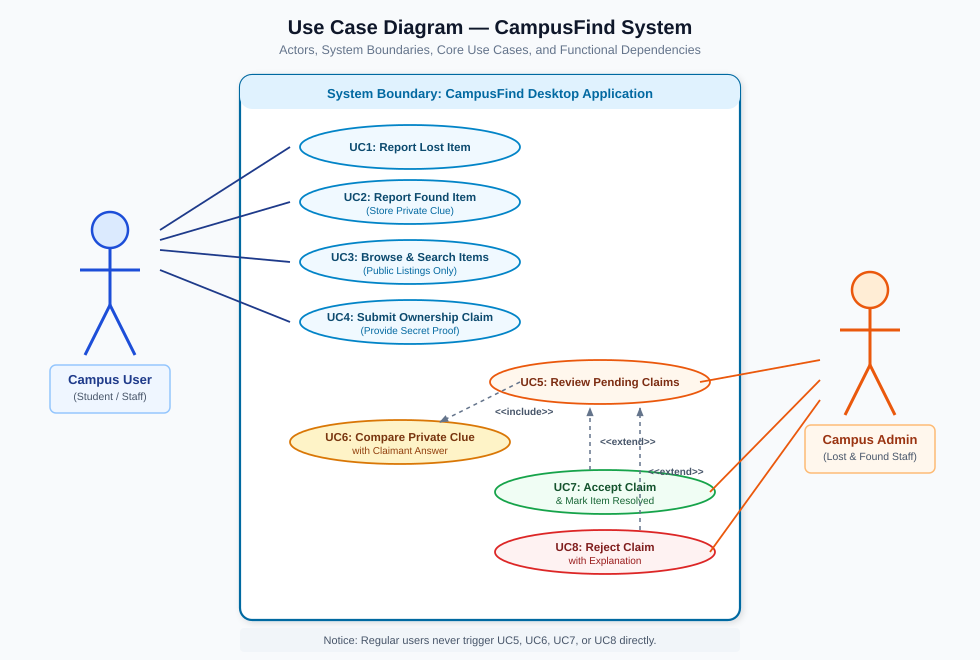
\includegraphics[width=0.88\textwidth]{diagrams/use-case.svg}}
    \caption{CampusFind Use Case Diagram}
    \label{fig:usecase}
\end{figure}

The primary operational use cases include:
\begin{itemize}
    \item \textbf{UC-1: Report Item (Lost / Found):} User selects classification, provides public details, and inputs private clue if item is found.
    \item \textbf{UC-2: Search Catalog:} User filters items by keywords or categories without exposing private attributes.
    \item \textbf{UC-3: Submit Claim:} User selects an open found item, inputs contact info and secret ownership proof.
    \item \textbf{UC-4: Review \& Adjudicate Claim:} Reviewer evaluates clue corroboration, enters remarks, and records decision.
\end{itemize}

% ==============================================================================
% 13. PROPOSED SYSTEM ARCHITECTURE
% ==============================================================================
\section{Proposed System Architecture}
CampusFind adopts a clear, beginner-friendly \textbf{Three-Tier Layered Architecture}:
\begin{enumerate}
    \item \textbf{Presentation Layer (\texttt{MainFrame}, \texttt{ItemTableModel}):} Renders the desktop GUI, handles user inputs, and delegates business operations to the service layer.
    \item \textbf{Business Logic Layer (\texttt{RecoveryService}):} Manages business rules, coordinates ID generation, performs input validation, and manages claim resolution workflows.
    \item \textbf{Persistence Layer (\texttt{FileStorage}, CSV Files):} Implements file-based reading, writing, and CSV parsing for \texttt{Item} and \texttt{Claim} entities.
\end{enumerate}

% ==============================================================================
% 14. DATA MODEL AND STORAGE APPROACH
% ==============================================================================
\section{Data Model and Data Storage Approach}
Data is modeled relationally at the logical level and implemented via lightweight CSV flat files:
\begin{itemize}
    \item \texttt{data/items.csv}: \texttt{itemId, itemType, title, category, publicDescription, location, reportDate, contactInfo, privateClue, itemStatus}
    \item \texttt{data/claims.csv}: \texttt{claimId, itemId, claimantName, claimantContact, ownershipAnswer, claimStatus, submissionDate, reviewNotes}
\end{itemize}
Foreign-key integrity between \texttt{Claim.itemId} and \texttt{Item.itemId} is enforced programmatically within \texttt{RecoveryService}.

% ==============================================================================
% 15. SELECTED SOFTWARE PROCESS MODEL
% ==============================================================================
\section{Selected Software Process Model}
The project adopts an \textbf{Iterative and Incremental Development Model with Early UI Prototyping}~\cite{sommerville2016, pressman2014}. 

\textbf{Rationale for Beginner Java Implementation:}
\begin{itemize}
    \item \textbf{Manageable Increments:} Developing the model classes first, followed by storage, service logic, and finally the GUI prevents beginner cognitive overload.
    \item \textbf{Early Stakeholder Feedback:} Creating visual UI mockups in Iteration 2 confirmed workflow requirements before code implementation.
    \item \textbf{Iterative Verification:} Automated unit testing at each stage ensures that regressions are caught immediately.
\end{itemize}

% ==============================================================================
% 16. DEVELOPMENT PHASES AND RATIONALE
% ==============================================================================
\section{Development Phases and Rationale}
\begin{enumerate}
    \item \textbf{Inception (Week 1):} Problem definition, requirements capture, stakeholder matrix.
    \item \textbf{Elaboration \& Modeling (Weeks 2--3):} DFD, Use Case, Activity, ERD, and Class diagram design; UI mockups.
    \item \textbf{Construction — Core Backend (Week 4):} Implementation of \texttt{Item}, \texttt{Claim}, \texttt{FileStorage}, and \texttt{RecoveryService}.
    \item \textbf{Construction — GUI \& Integration (Week 5):} Development of \texttt{MainFrame}, \texttt{ItemTableModel}, and verification workflow.
    \item \textbf{Transition \& Defense (Week 6):} Automated testing, defect resolution, proposal finalization, and repository publication.
\end{enumerate}

% ==============================================================================
% 17. PROJECT SCHEDULE AND MILESTONES
% ==============================================================================
\section{Project Schedule and Milestones}
\begin{table}[H]
    \centering
    \caption{Capstone Project Milestones and Completion Conditions}
    \begin{tabularx}{\textwidth}{llX}
        \toprule
        \textbf{Milestone} & \textbf{Target} & \textbf{Completion Condition} \\
        \midrule
        \textbf{M1} & Week 1 & Requirements specification and proposal scope signed off. \\
        \textbf{M2} & Week 2 & Complete UML diagram suite (DFD, Use Case, Activity, ERD) reviewed. \\
        \textbf{M3} & Week 3 & Class diagram, object snapshot, and UI prototypes finalized. \\
        \textbf{M4} & Week 4 & Core domain models, CSV storage engine, and service logic compiled. \\
        \textbf{M5} & Week 5 & Desktop Swing interface operational; automated test suite reports 10/10 PASS. \\
        \textbf{M6} & Week 6 & Proposal document compiled, web landing page published, repository ready. \\
        \bottomrule
    \end{tabularx}
\end{table}

% ==============================================================================
% 18. GANTT CHART
% ==============================================================================
\section{Gantt Chart}
\begin{table}[H]
    \centering
    \caption{Six-Week Capstone Engineering Schedule}
    \begin{tabularx}{\textwidth}{lcccccc}
        \toprule
        \textbf{Engineering Activity} & \textbf{W1} & \textbf{W2} & \textbf{W3} & \textbf{W4} & \textbf{W5} & \textbf{W6} \\
        \midrule
        Requirements \& Problem Definition & $\blacksquare$ & & & & & \\
        DFD (Level 0/1) \& Use Case Analysis & & $\blacksquare$ & & & & \\
        Activity Diagram \& Logical ERD Modeling & & $\blacksquare$ & $\blacksquare$ & & & \\
        Class Diagram \& Interface Wireframing & & & $\blacksquare$ & & & \\
        Backend Java Implementation (Model, Storage) & & & & $\blacksquare$ & & \\
        Service Business Logic \& ID Generators & & & & $\blacksquare$ & & \\
        Swing GUI (\texttt{MainFrame}, \texttt{ItemTableModel}) & & & & & $\blacksquare$ & \\
        Automated SQA Testing (10 Test Cases) & & & & & $\blacksquare$ & \\
        LaTeX Proposal, Documentation, Landing Page & & & & & & $\blacksquare$ \\
        Repository Configuration \& Defense Prep & & & & & & $\blacksquare$ \\
        \bottomrule
    \end{tabularx}
\end{table}

% ==============================================================================
% 19. DELIVERABLES AND ACCEPTANCE CRITERIA
% ==============================================================================
\section{Deliverables and Acceptance Criteria}
\begin{table}[H]
    \centering
    \caption{Project Deliverables and Verification Status}
    \begin{tabularx}{\textwidth}{lXll}
        \toprule
        \textbf{ID} & \textbf{Deliverable Description} & \textbf{Format / Location} & \textbf{Status} \\
        \midrule
        \textbf{D-1} & Formal Capstone Proposal Document & \texttt{proposal.tex} / \texttt{proposal.md} & Complete \\
        \textbf{D-2} & UML \& Software Diagram Suite & \texttt{proposal/diagrams/} (SVG/PUML) & Complete \\
        \textbf{D-3} & Interface Prototype Wireframes & \texttt{proposal/screenshots/} (SVG) & Complete \\
        \textbf{D-4} & Seven Java Source Classes & \texttt{src/campusfind/*.java} & Verified \\
        \textbf{D-5} & Automated Test Suite (10 Tests) & \texttt{CampusFindTestRunner.java} & 100\% Pass \\
        \textbf{D-6} & Web Landing Page & \texttt{website/index.html} & Published \\
        \bottomrule
    \end{tabularx}
\end{table}

% ==============================================================================
% 20. ALL REQUIRED UML / SOFTWARE DIAGRAMS
% ==============================================================================
\section{All Required UML and Software Engineering Diagrams}

\subsection{Data Flow Diagram (DFD) — Level 0 Context}
Figure~\ref{fig:dfd0} illustrates the system boundary, external entities (\textit{Campus User} and \textit{Campus Administrator}), and bidirectional information flows.

\begin{figure}[H]
    \centering
    \fbox{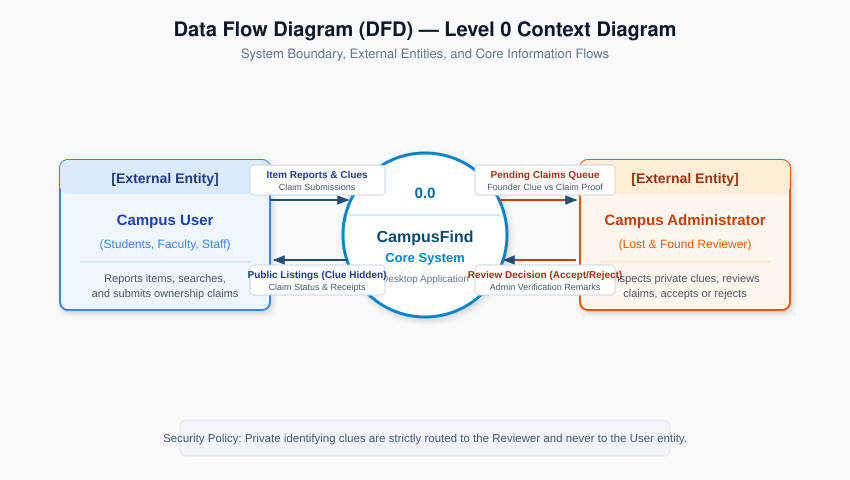
\includegraphics[width=0.85\textwidth]{diagrams/dfd-context.svg}}
    \caption{DFD Level 0 — Context Diagram}
    \label{fig:dfd0}
\end{figure}

\subsection{Data Flow Diagram (DFD) — Level 1 Decomposition}
Figure~\ref{fig:dfd1} decomposes the system into five sub-processes (1.0 Record Item, 2.0 Browse \& Search, 3.0 Submit Claim, 4.0 Verify Claims, 5.0 Resolve Item) and two internal data stores (\texttt{D1: Items Store} and \texttt{D2: Claims Store}).

\begin{figure}[H]
    \centering
    \fbox{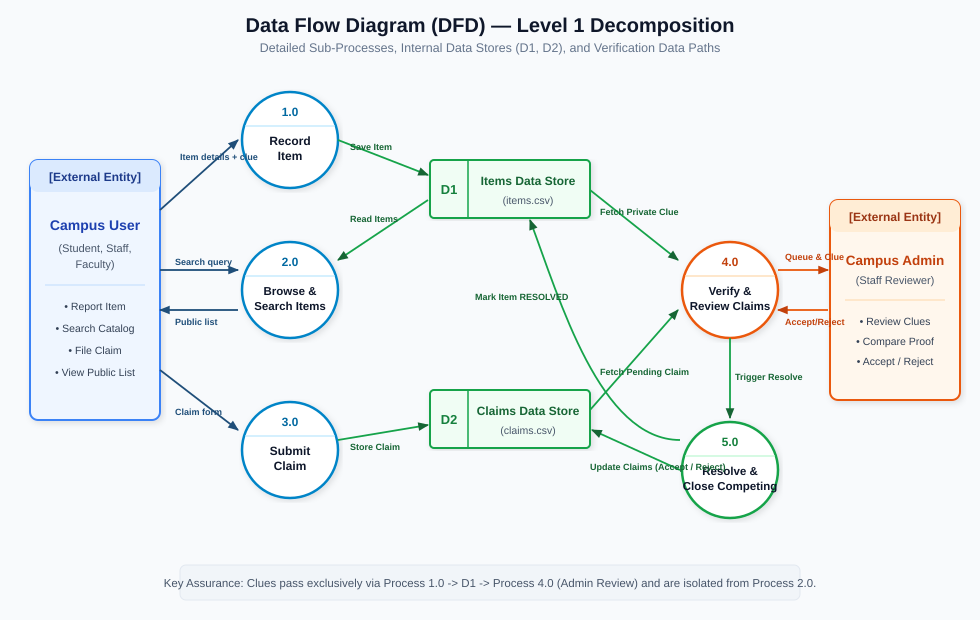
\includegraphics[width=0.9\textwidth]{diagrams/dfd-level1.svg}}
    \caption{DFD Level 1 — Process Decomposition}
    \label{fig:dfd1}
\end{figure}

\subsection{Activity Diagram}
Figure~\ref{fig:activity} depicts the cross-functional swimlane workflow between the Claimant and Administrator, detailing validation decisions, side-by-side comparison, claim approval, auto-rejection of competing claims, and item resolution.

\begin{figure}[H]
    \centering
    \fbox{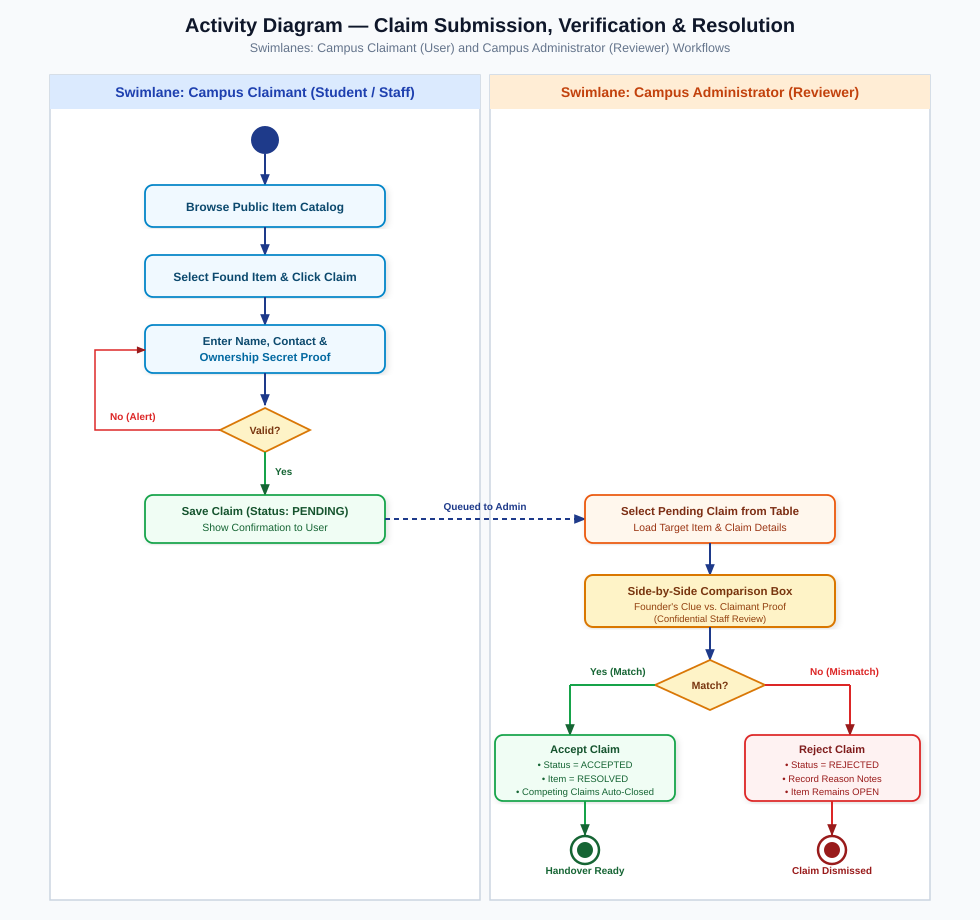
\includegraphics[width=0.85\textwidth]{diagrams/activity.svg}}
    \caption{Activity Diagram — Claim Submission and Verification Workflow}
    \label{fig:activity}
\end{figure}

\subsection{Entity Relationship Diagram (ERD)}
Figure~\ref{fig:erd} defines the conceptual relational data model, showing the $1:0..*$ cardinality between \texttt{ITEM} and \texttt{CLAIM}, primary keys, and foreign-key relationships.

\begin{figure}[H]
    \centering
    \fbox{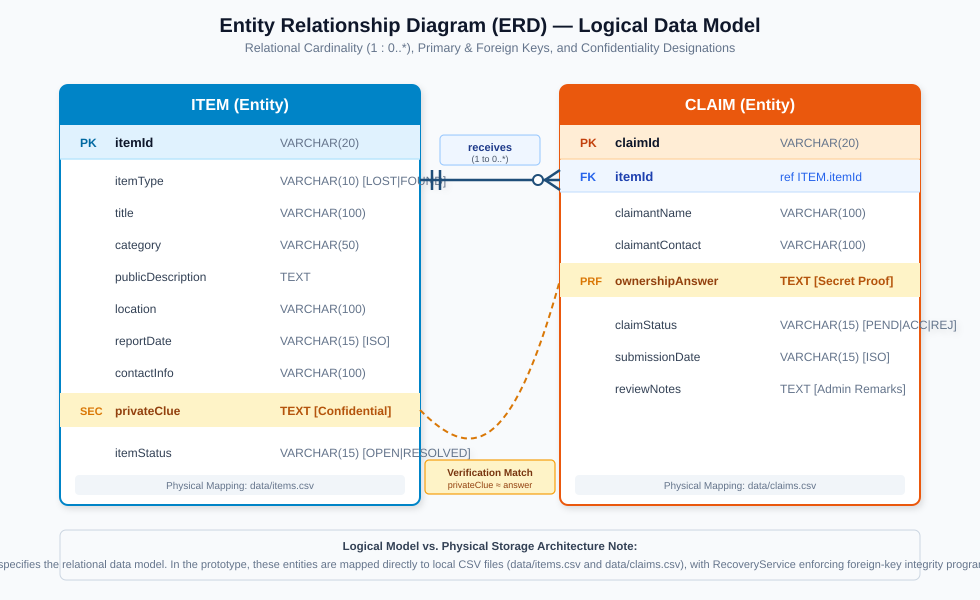
\includegraphics[width=0.9\textwidth]{diagrams/erd.svg}}
    \caption{Entity Relationship Diagram (ERD)}
    \label{fig:erd}
\end{figure}

\subsection{Class Diagram}
Figure~\ref{fig:class} displays the object-oriented structure matching the implemented Java classes (\texttt{Main}, \texttt{MainFrame}, \texttt{Item}, \texttt{Claim}, \texttt{RecoveryService}, \texttt{FileStorage}, and \texttt{ItemTableModel}).

\begin{figure}[H]
    \centering
    \fbox{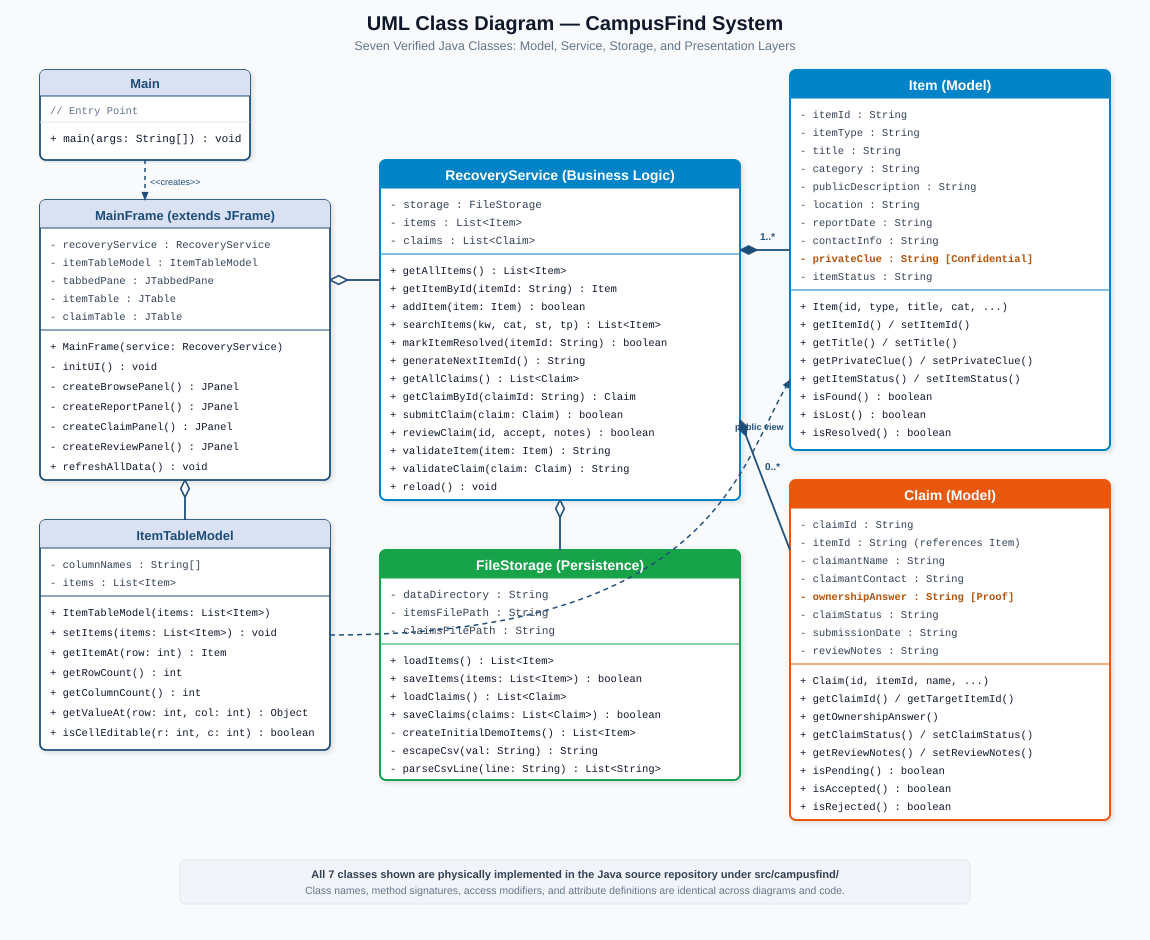
\includegraphics[width=0.95\textwidth]{diagrams/class-diagram.svg}}
    \caption{UML Class Diagram — Implemented System Architecture}
    \label{fig:class}
\end{figure}

\subsection{Object Diagram}
Figure~\ref{fig:object} captures a concrete runtime snapshot of concrete instances (\texttt{backpack: Item} and \texttt{claim1: Claim}), illustrating how the claimant's answer corroborates the founder's private clue.

\begin{figure}[H]
    \centering
    \fbox{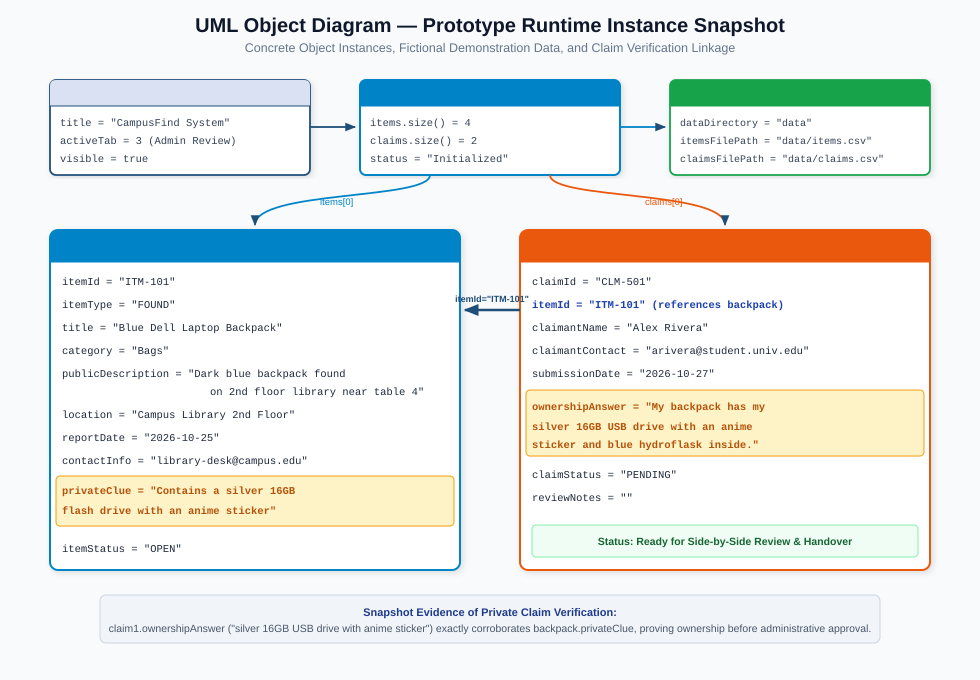
\includegraphics[width=0.9\textwidth]{diagrams/object-diagram.svg}}
    \caption{UML Object Diagram — Runtime Memory Snapshot}
    \label{fig:object}
\end{figure}

% ==============================================================================
% 21. INTERFACE PROTOTYPE AND SCREENSHOTS
% ==============================================================================
\section{Interface Prototype Description and Screenshots}

\begin{figure}[H]
    \centering
    \fbox{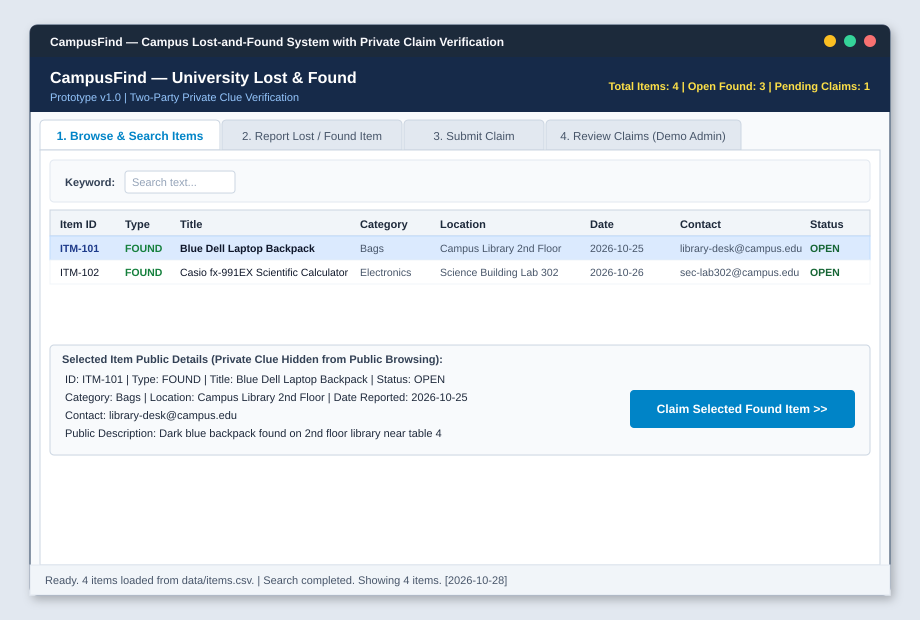
\includegraphics[width=0.88\textwidth]{screenshots/ui-browse.svg}}
    \caption{Tab 1: Browse and Search Items Screen}
    \label{fig:ui-browse}
\end{figure}
\textit{Explanation of Figure~\ref{fig:ui-browse}:} The public browsing tab provides keyword, category, type, and status filtering. As shown, table columns terminate at Status; private clues are strictly withheld. Clicking ``Claim Selected Found Item'' automatically transfers the item ID to Tab~3.

\begin{figure}[H]
    \centering
    \fbox{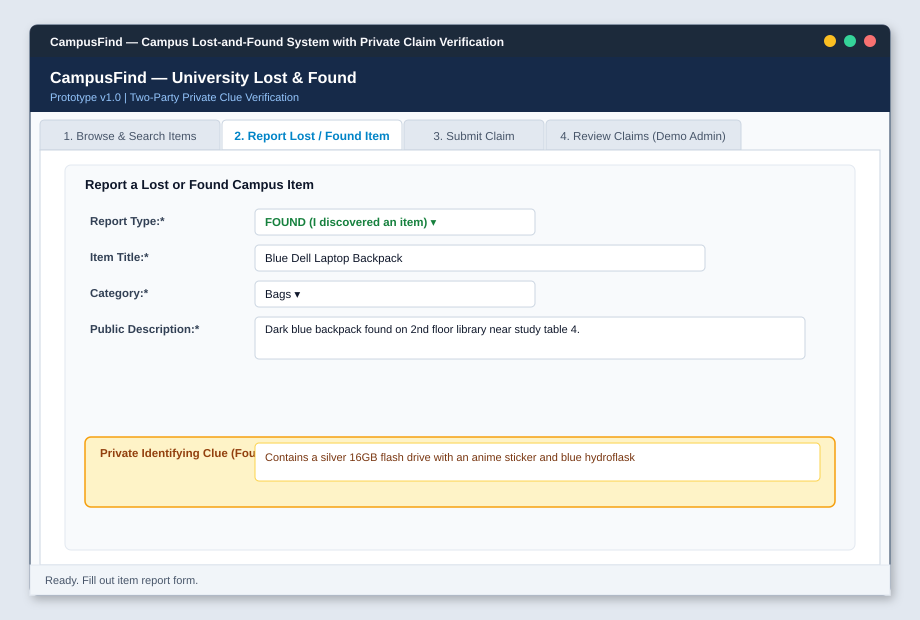
\includegraphics[width=0.88\textwidth]{screenshots/ui-report.svg}}
    \caption{Tab 2: Report Lost or Found Item Screen}
    \label{fig:ui-report}
\end{figure}
\textit{Explanation of Figure~\ref{fig:ui-report}:} The reporting screen enables campus members to register lost or found property. The highlighted amber panel captures confidential identifying clues for found items.

\begin{figure}[H]
    \centering
    \fbox{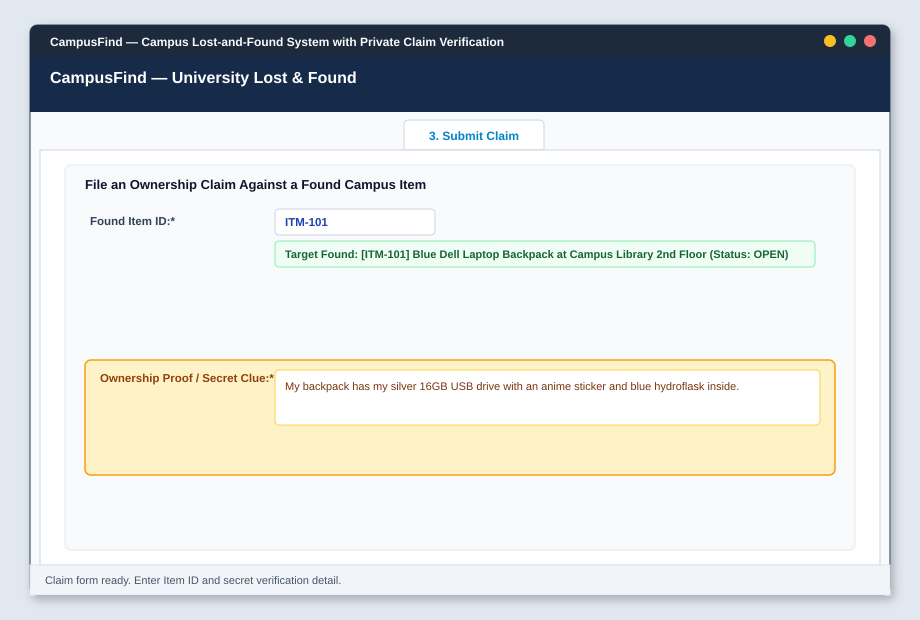
\includegraphics[width=0.88\textwidth]{screenshots/ui-claim.svg}}
    \caption{Tab 3: Submit Ownership Claim Screen}
    \label{fig:ui-claim}
\end{figure}
\textit{Explanation of Figure~\ref{fig:ui-claim}:} The claim filing tab validates the target item ID, displays an item confirmation badge, and captures the claimant's secret corroboration proof.

\begin{figure}[H]
    \centering
    \fbox{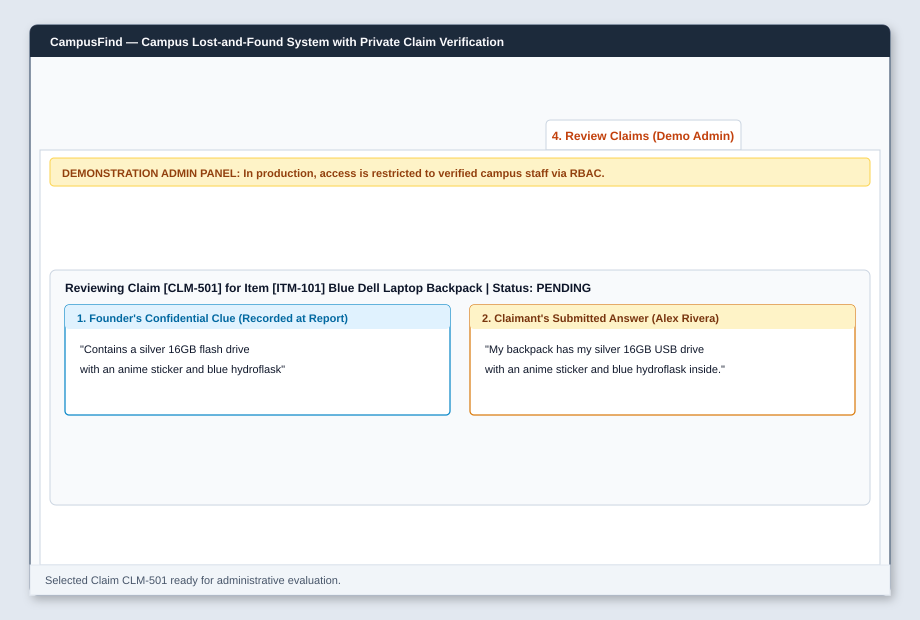
\includegraphics[width=0.88\textwidth]{screenshots/ui-review.svg}}
    \caption{Tab 4: Review Claims (Demo Admin) Screen}
    \label{fig:ui-review}
\end{figure}
\textit{Explanation of Figure~\ref{fig:ui-review}:} The staff verification console displays the founder's confidential clue side-by-side with the claimant's submitted proof, enabling evidence-based approval or rejection.

% ==============================================================================
% 22. TESTING STRATEGY AND TEST CASES
% ==============================================================================
\section{Testing Strategy and Test Cases}
The testing strategy combines automated headless execution via \texttt{CampusFindTestRunner.java} with interactive Swing UI validation. Table~\ref{tab:testcases} outlines the verified test matrix.

\begin{table}[H]
    \centering
    \caption{Automated Verification Test Matrix}
    \label{tab:testcases}
    \begin{tabularx}{\textwidth}{lp{4cm}Xl}
        \toprule
        \textbf{ID} & \textbf{Test Description} & \textbf{Expected Result} & \textbf{Status} \\
        \midrule
        \textbf{TC-01} & Demo Data Seeding & Missing CSV files auto-seeded with 4 items, 2 claims. & \textbf{PASS} \\
        \textbf{TC-02} & Record Lost Item & Item recorded with status OPEN and sequential ID. & \textbf{PASS} \\
        \textbf{TC-03} & Record Found Item + Clue & Private clue recorded and persisted. & \textbf{PASS} \\
        \textbf{TC-04} & Information Hiding & Table model strictly omits clue columns and values. & \textbf{PASS} \\
        \textbf{TC-05} & Multi-Criteria Search & Search filters return accurate matching subsets. & \textbf{PASS} \\
        \textbf{TC-06} & Submit Valid Claim & Claim saved with status PENDING linked to item. & \textbf{PASS} \\
        \textbf{TC-07} & Validation Rules & Blank claimant names or invalid IDs rejected. & \textbf{PASS} \\
        \textbf{TC-08} & Review and Reject Claim & Claim status updated to REJECTED with notes. & \textbf{PASS} \\
        \textbf{TC-09} & Accept Claim (Auto-Resolve) & Item marked RESOLVED; competing claims auto-closed. & \textbf{PASS} \\
        \textbf{TC-10} & Local Storage Reload & Fresh instance loads persisted CSV data accurately. & \textbf{PASS} \\
        \bottomrule
    \end{tabularx}
\end{table}

% ==============================================================================
% 23. FEASIBILITY ANALYSIS
% ==============================================================================
\section{Feasibility Analysis}
\begin{itemize}
    \item \textbf{Technical Feasibility:} Highly feasible. The system relies exclusively on the standard Java SE runtime environment (JDK 8+), requiring no paid servers or complex frameworks.
    \item \textbf{Operational Feasibility:} Highly feasible. The tabbed desktop interface requires minimal user training; campus staff can immediately perform claim reviews.
    \item \textbf{Schedule Feasibility:} Highly feasible. The six-week incremental development plan accommodates prototype completion, testing, and documentation within semester deadlines.
    \item \textbf{Cost Feasibility:} Optimal feasibility. Development and runtime costs are \$0 due to open-source tooling, local file storage, and GitHub hosting.
\end{itemize}

% ==============================================================================
% 24. RISK ANALYSIS AND MITIGATION
% ==============================================================================
\section{Risk Analysis and Mitigation}
\begin{table}[H]
    \centering
    \caption{Risk Matrix and Mitigation Strategies}
    \begin{tabularx}{\textwidth}{lp{3.5cm}cp{5.5cm}}
        \toprule
        \textbf{Risk ID} & \textbf{Identified Risk} & \textbf{Severity} & \textbf{Mitigation Strategy} \\
        \midrule
        \textbf{R-1} & CSV Data Corruption from Commas & Medium & Implement quote-wrapping and character-level CSV parsing in \texttt{FileStorage.java}. \\
        \textbf{R-2} & Accidental Clue Leakage & Critical & Filter attributes at the data model level (\texttt{ItemTableModel}) rather than relying solely on UI column hiding. \\
        \textbf{R-3} & Concurrent Competing Claims & Medium & Programmatic business rule in \texttt{RecoveryService} auto-rejects pending competing claims upon approval of a verified claim. \\
        \bottomrule
    \end{tabularx}
\end{table}

% ==============================================================================
% 25. PRIVACY AND ETHICAL CONSIDERATIONS
% ==============================================================================
\section{Privacy and Ethical Considerations}
Campus lost-and-found items often contain sensitive personal data (e.g., student IDs, credit cards, laptop stickers). CampusFind incorporates the following privacy protections:
\begin{enumerate}
    \item \textbf{Data Minimization:} Demonstrations use fictional sample data exclusively; real student phone numbers or national IDs are never recorded.
    \item \textbf{Confidentiality of Secret Details:} Private clues are restricted to administrative review and never displayed in public listings or search queries.
    \item \textbf{Disclaimer Notice:} System documentation explicitly notes that production deployment would require full institutional access control and secure physical handovers.
\end{enumerate}

% ==============================================================================
% 26. EXPECTED OUTCOMES AND BENEFITS
% ==============================================================================
\section{Expected Outcomes and Benefits}
\begin{itemize}
    \item Improved campus recovery rates through centralized public item searching.
    \item Significant reduction in fraudulent property claims due to two-party private clue corroboration.
    \item Transparent administrative audit trails with recorded review remarks.
    \item A clean, maintainable Java software engineering reference project for academic evaluation.
\end{itemize}

% ==============================================================================
% 27. FUTURE ENHANCEMENTS
% ==============================================================================
\section{Future Enhancements (Part II Roadmap)}
\begin{itemize}
    \item Migration from local CSV storage to an embedded relational database (SQLite/PostgreSQL).
    \item Institutional Single Sign-On (SSO) integration with role-based access control (RBAC).
    \item Automated email notifications alerting claimants upon review decisions.
    \item Integration with smart campus lockers for automated after-hours item pickup.
\end{itemize}

% ==============================================================================
% 28. CONCLUSION
% ==============================================================================
\section{Conclusion}
The CampusFind capstone project demonstrates that rigorous Software Engineering deliverables—system modeling, process planning, requirements specification, and quality assurance—can be achieved using straightforward, beginner-friendly Java fundamentals. By implementing two-tier private claim verification, the application solves a genuine university operational challenge without unnecessary architectural complexity. All deliverables, diagrams, source classes, and test suites are fully realized and ready for academic submission.

% ==============================================================================
% 29. REFERENCES
% ==============================================================================
\section{References}
\begin{enumerate}
    \item Sommerville, I. (2016). \textit{Software Engineering} (10th ed.). Pearson. \url{https://www.pearson.com}
    \item Pressman, R. S., \& Maxim, B. R. (2014). \textit{Software Engineering: A Practitioner's Approach} (8th ed.). McGraw-Hill Education.
    \item Fowler, M. (2003). \textit{UML Distilled: A Brief Guide to the Standard Object Modeling Language} (3rd ed.). Addison-Wesley Professional.
    \item Larman, C. (2004). \textit{Applying UML and Patterns: An Introduction to Object-Oriented Analysis and Design} (3rd ed.). Prentice Hall.
    \item Oracle Corporation. (2024). \textit{Java Platform, Standard Edition Documentation}. \url{https://docs.oracle.com/en/java/javase/}
    \item Oracle Corporation. (2024). \textit{Creating a GUI With Swing (The Java Tutorials)}. \url{https://docs.oracle.com/javase/tutorial/uiswing/}
    \item IEEE Computer Society. (1998). \textit{IEEE Recommended Practice for Software Requirements Specifications} (IEEE Std 830-1998). \url{https://standards.ieee.org}
\end{enumerate}

% ==============================================================================
% 30. APPENDIX
% ==============================================================================
\appendix
\section{Appendix: Beginner Class Walkthrough and Demonstration Script}
\subsection{Class Responsibilities Summary}
\begin{itemize}
    \item \texttt{Main.java}: Application entry point; initializes dependencies and schedules GUI launch on the Swing Event Dispatch Thread (EDT).
    \item \texttt{Item.java}: Domain model representing lost and found items, encapsulating public fields and confidential clues.
    \item \texttt{Claim.java}: Domain model representing submitted ownership claims and verification status.
    \item \texttt{FileStorage.java}: Manages local CSV file persistence and initial demo data seeding.
    \item \texttt{RecoveryService.java}: Business logic service enforcing validation rules, ID sequencing, and lifecycle resolution.
    \item \texttt{ItemTableModel.java}: Swing TableModel strictly enforcing information hiding for public catalog queries.
    \item \texttt{MainFrame.java}: Graphical user interface containing the four primary operational tabs.
    \item \texttt{CampusFindTestRunner.java}: Headless automated SQA test suite executing ten verification test cases.
\end{itemize}

\subsection{Standard Compilation and Run Commands}
\begin{lstlisting}[language=bash]
# 1. Compile all Java source classes into the bin/ directory
javac -d bin src/campusfind/*.java

# 2. Run the graphical desktop application
java -cp bin campusfind.Main

# 3. Run the automated headless QA verification test suite
java -cp bin campusfind.CampusFindTestRunner
\end{lstlisting}

\end{document}
